
% part 10
\section{Преобразованная поэзия\label{sec:part10}}

\subsection{Клиент 5.0}


Теперь мы будем добавлять некоторую трансформирующую логику в 
наш поэтический клиент к строкам, предложенным в части 9, с 
использованием упрощенного преобразования - Cummingsifier.
Cummingsifier - алгоритм, который на вход берет поэму и возвращает 
поэму в стиле \href{http://en.wikipedia.org/wiki/E.\_E.\_Cummings}{e.e.cummings}.
Далее алгоритм, который выполняет преoбразование:

\begin{scriptsize}\begin{verbatim}
def cummingsify(poem):
    return poem.lower()
\end{verbatim}\end{scriptsize} 

К сожалению, этот алгоритм очень простой и, реально нем никогда не произойдет ошибки, 
поэтому в клиенте 5.0, расположенном в 
\href{http://github.com/jdavisp3/twisted-intro/blob/master/twisted-client-5/get-poetry.py#L1}{twisted-client-5/get-poetry.py}, мы используем модифицированную версию 
cummingsify, которая произвольно выполняет следующее:

\begin{enumerate}
\item Возвращает трансформированную версию
\item Генерирует GibberishError
\item Генерирует ValueError
\end{enumerate}


Таким образом мы эмулируем более сложный алгоритм, который иногда может 
глючить.


Изменения в клиенте 5.0 также сделаны в функции poetry\_main:

\begin{scriptsize}\begin{verbatim}
def poetry_main():
    addresses = parse_args()

    from twisted.internet import reactor

    poems = []
    errors = []

    def try_to_cummingsify(poem):
        try:
            return cummingsify(poem)
        except GibberishError:
            raise
        except:
            print 'Cummingsify failed!'
            return poem

    def got_poem(poem):
        print poem
        poems.append(poem)

    def poem_failed(err):
        print >>sys.stderr, 'The poem download failed.'
        errors.append(err)

    def poem_done(_):
        if len(poems) + len(errors) == len(addresses):
            reactor.stop()

    for address in addresses:
        host, port = address
        d = get_poetry(host, port)
        d.addCallback(try_to_cummingsify)
        d.addCallbacks(got_poem, poem_failed)
        d.addBoth(poem_done)

    reactor.run()
\end{verbatim}\end{scriptsize}


Таким образом, когда программа скачивает поэму c сервера, она будет 
выполнять одно из:

\begin{enumerate}
\item Печатать трансформированную версию поэмы
\item Печатать “Cummingsify failed!” и оригинальную версию поэмы
\item Печатать “The poem download failed.” 
\end{enumerate}


Хотя мы сохранили возможность скачивать с нескольких серверов, 
когда вы будете проверять клиент 5.0, проще использовать один сервер и 
запускать программу несколько раз, до тех пор пока вы не увидите 
различные выводы. Также попробуйте запустить клиент с портом, на котором 
не запущен сервер.


Давайте нарисуем цепочку callback/errback, которые создаются для каждого 
Deferred'а, создаваемого в функции get\_poetry: 

% fig19
\begin{figure}[h]
\begin{center}
    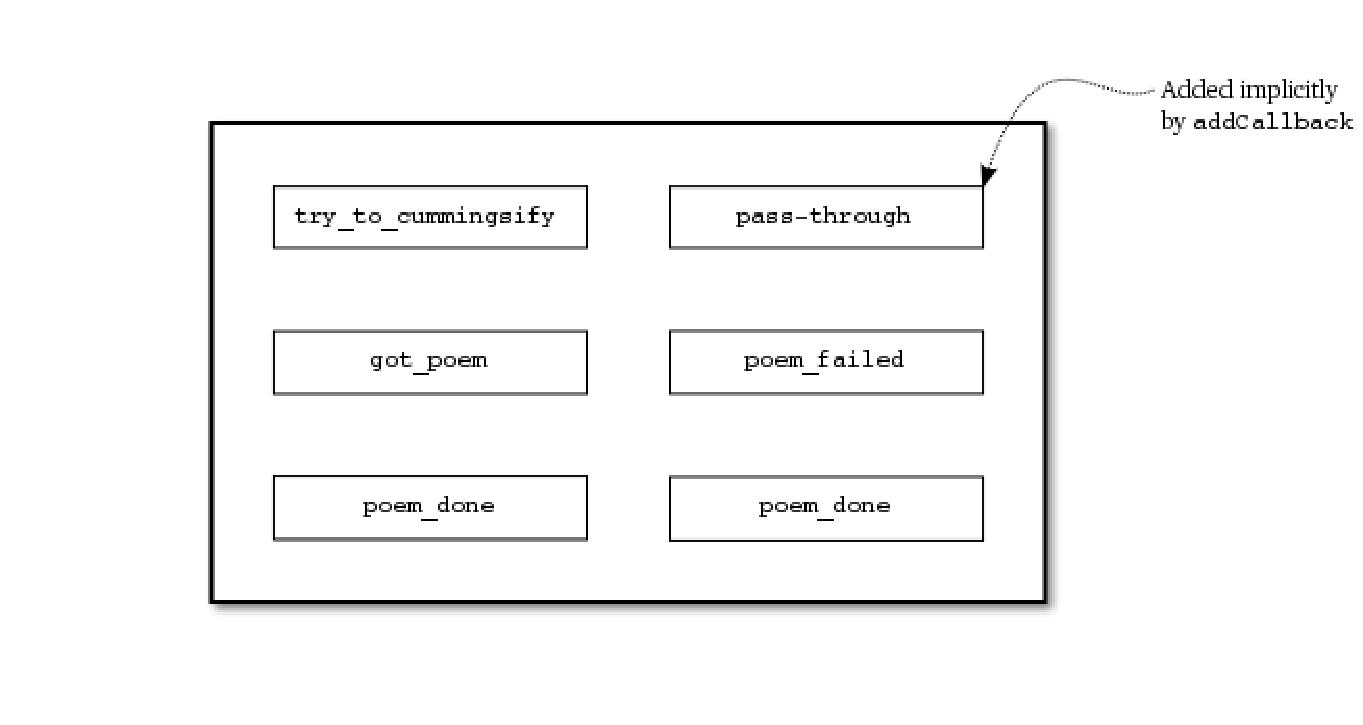
\includegraphics[width=0.8\textwidth]{images/deferred-42.pdf}
    \caption{Цепочка deferred'а в клиенте 5.0\label{fig:deferred-42}}
\end{center}
\end{figure}


Обратите внимание, что pass-through добавляется неявно в errback 
функцией addCallback. Функция pass-through ничего не делает и передает 
свой аргумент типа Failure следующему errback'у (poem\_failed). Таким образом, 
poem\_failed может управлять ошибками из двух функций: get\_poetry (в этом 
случае deferred poem\_failed активизируется предыдущим deferred'ом из цепочки 
errback) и функцией cummingsify.


Нужно заметить, что великолепная тень на рисунке \ref{fig:deferred-42} 
была сделана в \href{http://inkscape.org/}{Inkscape}\footnote[1]{http://inkscape.org/}.


Давайте проанализируем различные способы, которые могут активизировать наши deferred'ы.
Случай, когда мы получаем поэму и функция cummingsify работает корректно, изображен 
на рисунке \ref{fig:deferred-5}:

% fig20
\begin{figure}[h]
\begin{center}
    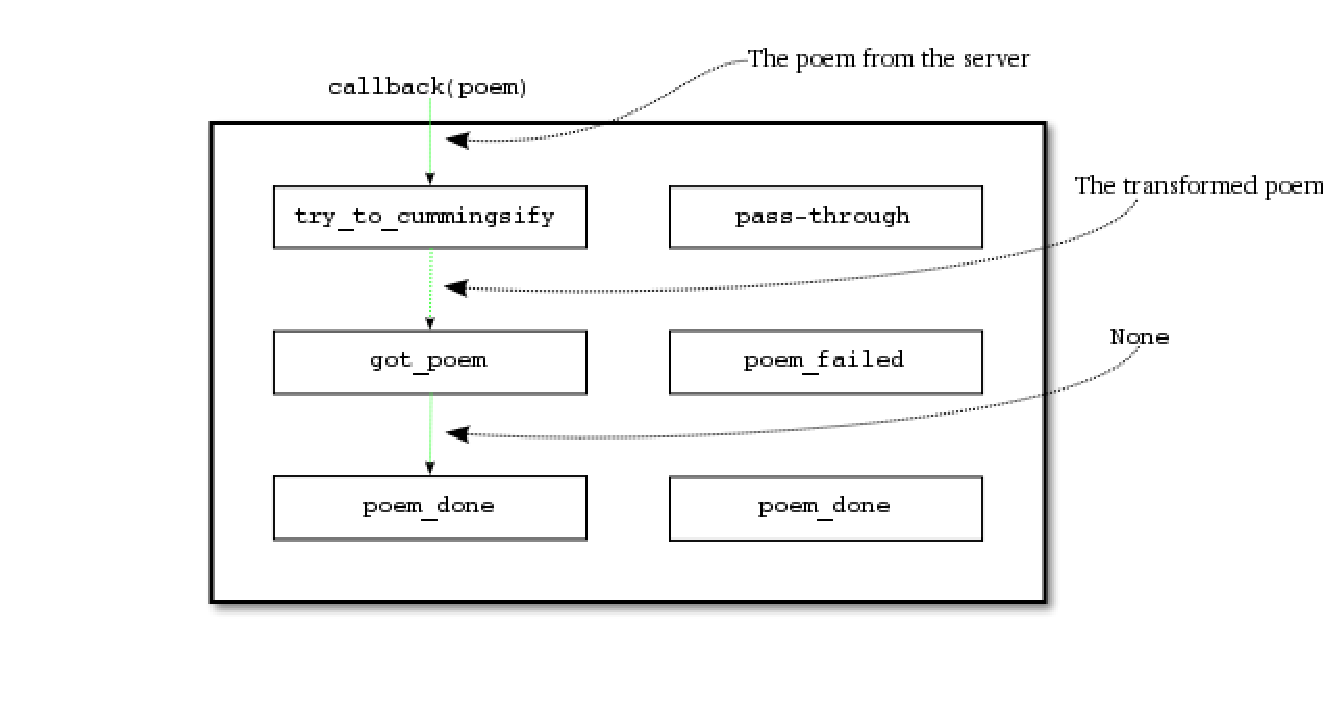
\includegraphics[width=0.8\textwidth]{images/deferred-5.pdf}
    \caption{Цепочка deferred'а в клиенте 5.0\label{fig:deferred-5}}
\end{center}
\end{figure}

В этом случае, ни в одном callback'е не произошло ошибок, так что 
управление полностью проходит вниз по линии callback. Заметим, что 
функция poem\_done получает None в качестве аргумета, поскольку 
got\_poem в действительности не возвращает значение. 
Если мы хотим, чтобы каждая функция из линии callback 
имела доступ к поэме, то нам нужно поменять функцию got\_poem так, 
чтобы она возвращала поэму.


Рисунок \ref{fig:deferred-6} иллюстрирует случай, когда мы получием поэму, но 
в функции cummingsify генерирует исключение GibberishError:

% fig21
\begin{figure}[h]
\begin{center}
    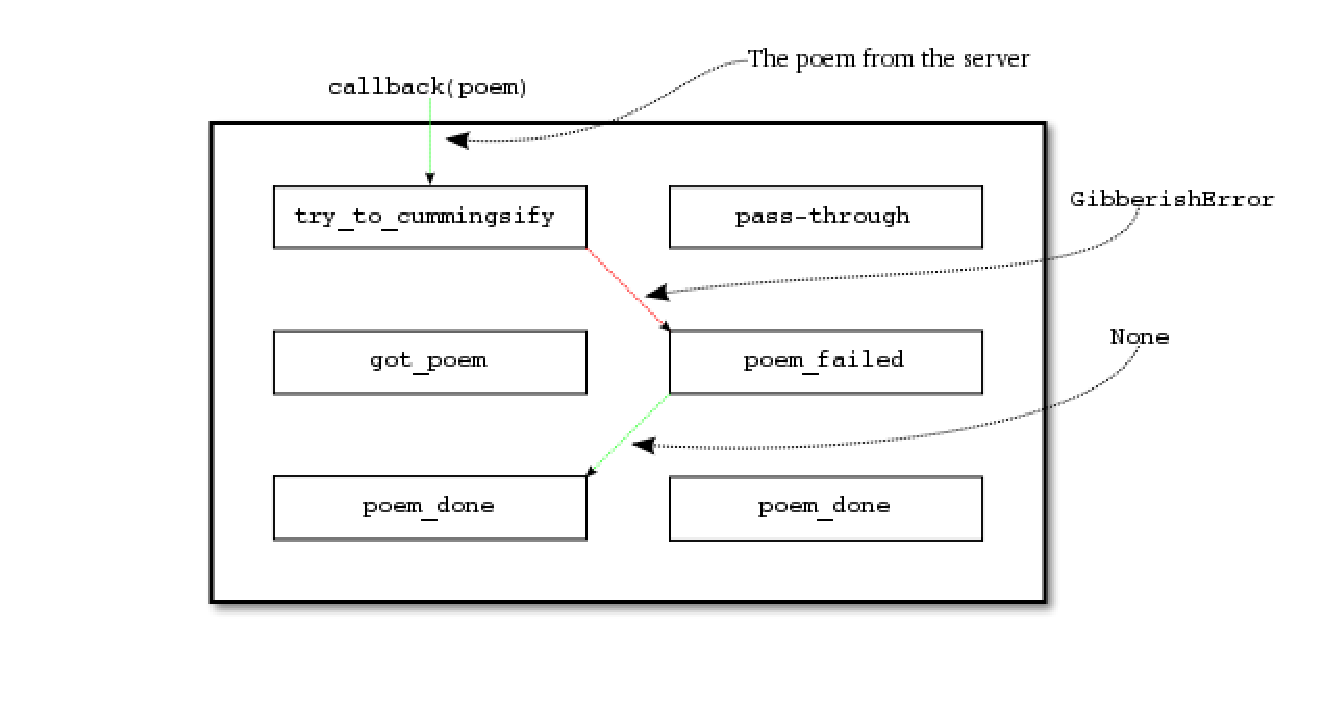
\includegraphics[width=0.8\textwidth]{images/deferred-6.pdf}
    \caption{Случай, когда мы скачали поэму и получили GibberishError\label{fig:deferred-6}}
\end{center}
\end{figure}


После того как try\_to\_cummingsify callback генерирует во второй раз 
ислючение GibberishError, управление переключается на линию errback и 
вызывается poem\_failed с исключением в качестве своего параметра (естественно, 
обернутого в Failure).


И, так как poem\_failed не вызывает исключение, или не возвращает Failure, 
то после того, как она завершит работу, контроль переключается обратно на линии 
callback. Если мы предполагаем, что poem\_failed полностью управляет ошибками, 
то возвратить None - это разумное поведение. С другой стороны, если мы хотим, чтобы 
poem\_failed производила некоторое дейтсвие, но все еще передавала ошибку, мы 
могли бы поменять poem\_failed так, чтобы она возвращала свой аргумент err и, 
обработка продолжилась бы ниже по линии errback. 


Заметим, что ни в got\_poem, ни в poem\_failed никогда не 
происходит ошибок, так что функция poem\_done для errback никогда не 
будет вызвана. Но, безопасней добавить добавить такую функцию в errback, 
чтобы явится примером ``оборонительного'' программирования, 
так как или got\_poem, или poem\_failed могут иметь ошибки, 
о которых мы не знаем. Так как метод addBoth гарантирует, что 
определенная функция запустится независимо от того как 
deferred был активизирован (ошибкой или результатом), использование addBoth  
является аналогичным добавлению finally в оператор try/except. 


Теперь исследуем случай, который изображен на рисунке \ref{fig:deferred-7}, 
когда мы скачали поэму, и функция cummingsify 
сгнерировала исключение ValueError.

% fig22
\begin{figure}[h]
\begin{center}
    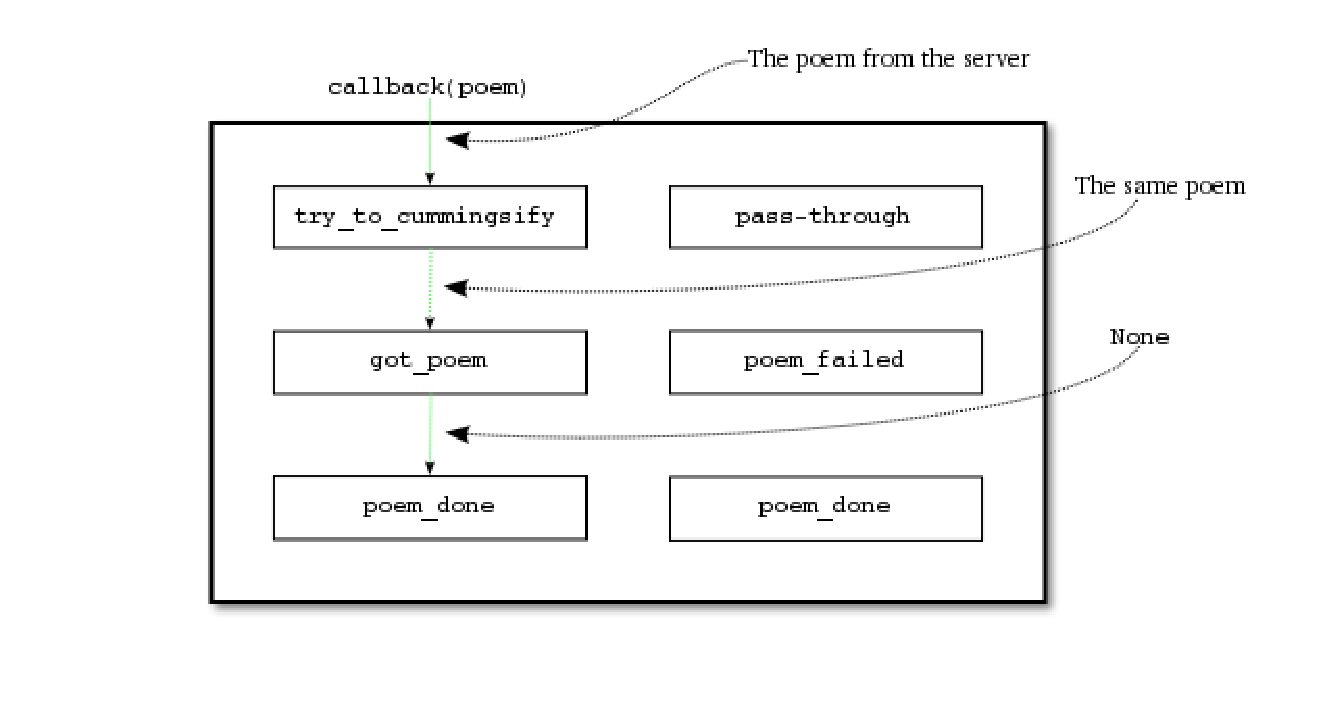
\includegraphics[width=0.8\textwidth]{images/deferred-7.pdf}
    \caption{Случай, когда мы скачали поэму и в cummingsify произошла ошибка\label{fig:deferred-7}}
\end{center}
\end{figure}


Эта ситуация аналогична ситуации на рисунку \ref{fig:deferred-5}, 
за исключением, что got\_poem получает оригинальную версию поэмы 
вместо трансформированной версии. Переключение происходит полностью 
внутри callback'а try\_to\_cummingsify, который отлавливает 
исключение ValueError обычным оператором try/except и возвращает 
оригинальную поэму. Объект deferred не обнаруживает ошибки.


И наконец, рисунок \ref{fig:deferred-8} - мы рассматриваем случай, когда мы пытались скачать 
поэму из несуществующего сервера:

% fig23
\begin{figure}[h]
\begin{center}
    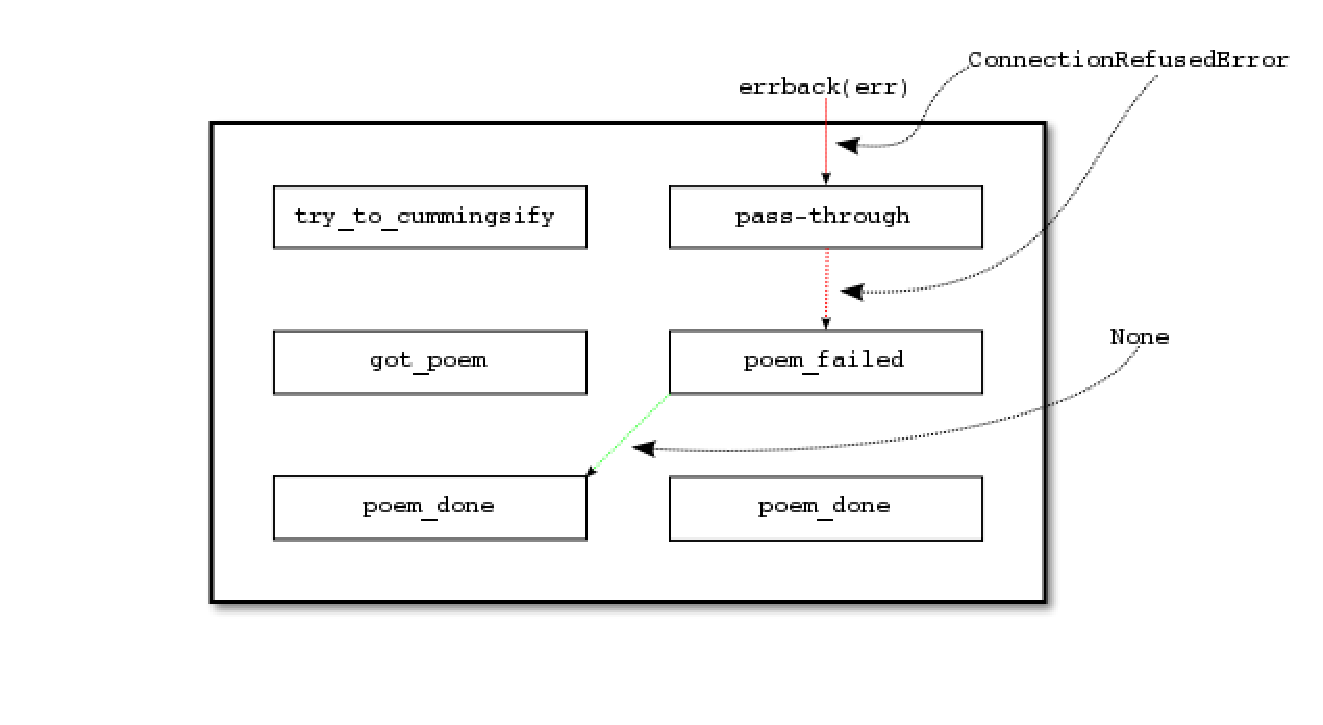
\includegraphics[width=0.8\textwidth]{images/deferred-8.pdf}
    \caption{Случай, когда мы не можем соединиться с сервером\label{fig:deferred-8}}
\end{center}
\end{figure}


Как и прежде, poem\_failed возвращает None, поэтому далее контроль переключается на 
линию callback.

\subsection{Клиент 5.1}


В клиенте 5.0 мы отлавливаем исключение из функции cummingsify в 
нашем callback'е try\_to\_cummingsify, используя обычный оператор 
try/except, не позволяя deferred'у ловить его первым. Такой подход 
не является обязательно ошибычным, но является поучительным рассмотреть 
как мы можем сделать это по-другому.  


Давайте предположим, что мы хотим позволить deferred'у ловить 
оба исключения GibberishError и ValueError и отправлять их 
по цепи errback. Для того, чтобы сохранить поведение нашей 
последовательности errback, нужно проверить: если мы видим, что 
ошибка ValueError, то нужно возвратить оригинальную поэму, так чтобы 
управление вернулось обратно на цепь callback и, чтобы оригинальная 
поэма напечаталась.


Но здесь есть проблема: errback не получил бы оригинальную поэму, 
вместо этого получил бы завернунутое в Failure исключение ValueError, 
сгенерированное функцией cummingsify. Для того, чтобы позволить 
errback управлять ошибкой, нам нужно сделать так, чтобы errback получал 
оригинальную поэму.


Один из способов сделать такое - это поменять функцию cummingsify так, чтобы 
оригинальная поэма была добавлена в исключение. Это то, что мы сделали в клиенте 5.1, 
расположенном в 
\href{http://github.com/jdavisp3/twisted-intro/blob/master/twisted-client-5/get-poetry-1.py#L1}{twisted-client-5/get-poetry-1.py}. Мы поменяли исключение ValueError на специальное исключение CannotCummingsify, которое 
принимает оригинальную поэму в качестве своего первого аргумента. 


Если бы cummingsify была бы реальной функцией во внешнем модуле, 
то, вероятно, лучшим решением было бы обернуть ее другой функцией, 
которая отлавливала бы любое исключение кроме GibberishError 
и генерировала бы исключение CannotCummingsify. С нашей новой 
структурой, функция poetry\_main выглядит так:

\begin{scriptsize}\begin{verbatim}
def poetry_main():
    addresses = parse_args()

    from twisted.internet import reactor

    poems = []
    errors = []

    def cummingsify_failed(err):
        if err.check(CannotCummingsify):
            print 'Cummingsify failed!'
            return err.value.args[0]
        return err

    def got_poem(poem):
        print poem
        poems.append(poem)

    def poem_failed(err):
        print >>sys.stderr, 'The poem download failed.'
        errors.append(err)

    def poem_done(_):
        if len(poems) + len(errors) == len(addresses):
            reactor.stop()

    for address in addresses:
        host, port = address
        d = get_poetry(host, port)
        d.addCallback(cummingsify)
        d.addErrback(cummingsify_failed)
        d.addCallbacks(got_poem, poem_failed)
        d.addBoth(poem_done)
\end{verbatim}\end{scriptsize}

И каждый deferred имеет структуру как на рисунке \ref{fig:deferred-9}:
 
% fig24
\begin{figure}[h]
\begin{center}
    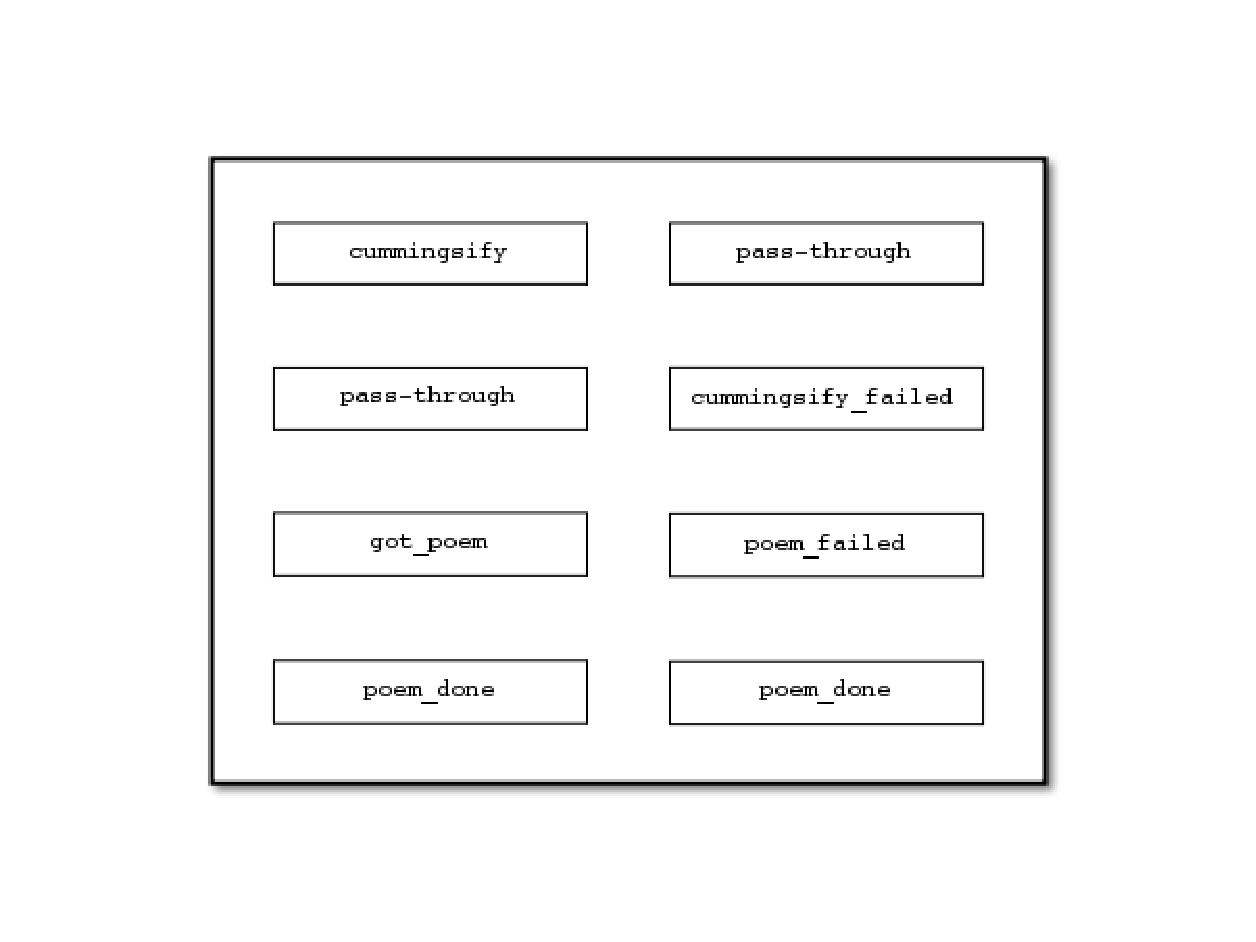
\includegraphics[width=0.8\textwidth]{images/deferred-9.pdf}
    \caption{Цепочка deferred'а в клиенте 5.1\label{fig:deferred-9}}
\end{center}
\end{figure}

Исследуем cummingsify\_failed errback:

\begin{scriptsize}\begin{verbatim}
    def cummingsify_failed(err):
        if err.check(CannotCummingsify):
            print 'Cummingsify failed!'
            return err.value.args[0]
        return err
\end{verbatim}\end{scriptsize}

%We are using the check method on Failure objects to test whether the exception embedded in the Failure is an instance of CannotCummingsify. If so, we return the first argument to the exception (the original poem) and thus handle the error. Since the return value is not a Failure, control returns to the callback line. Otherwise, we return the Failure itself and send (re-raise) the error down the errback line. As you can see, the exception is available as the value attribute on the Failure.

Мы используем метод check объектов типа Failure для проверки 
является ли исключение, встроенное в Failure экземпляром 
типа CannotCummingsify. Если это так, то мы возвращаем 
первый аргумент исключения (изначальную поэму) и, таким 
образом управляем ошибкой. Поскольку возвращаемое значение 
не является Failure, то контроль возвращается цепи callback. 
Иначе, мы возвращаем Failure и отправляем ошибку далее по 
цепи errback. Как вы можете это видеть, исключение доступно 
как значение атрибута объекта Failure.   


На рисунке \ref{fig:deferred-10} показано что случится, 
если мы получим исключение CannotCummingsify:

% fig25 
\begin{figure}[h]
\begin{center}
    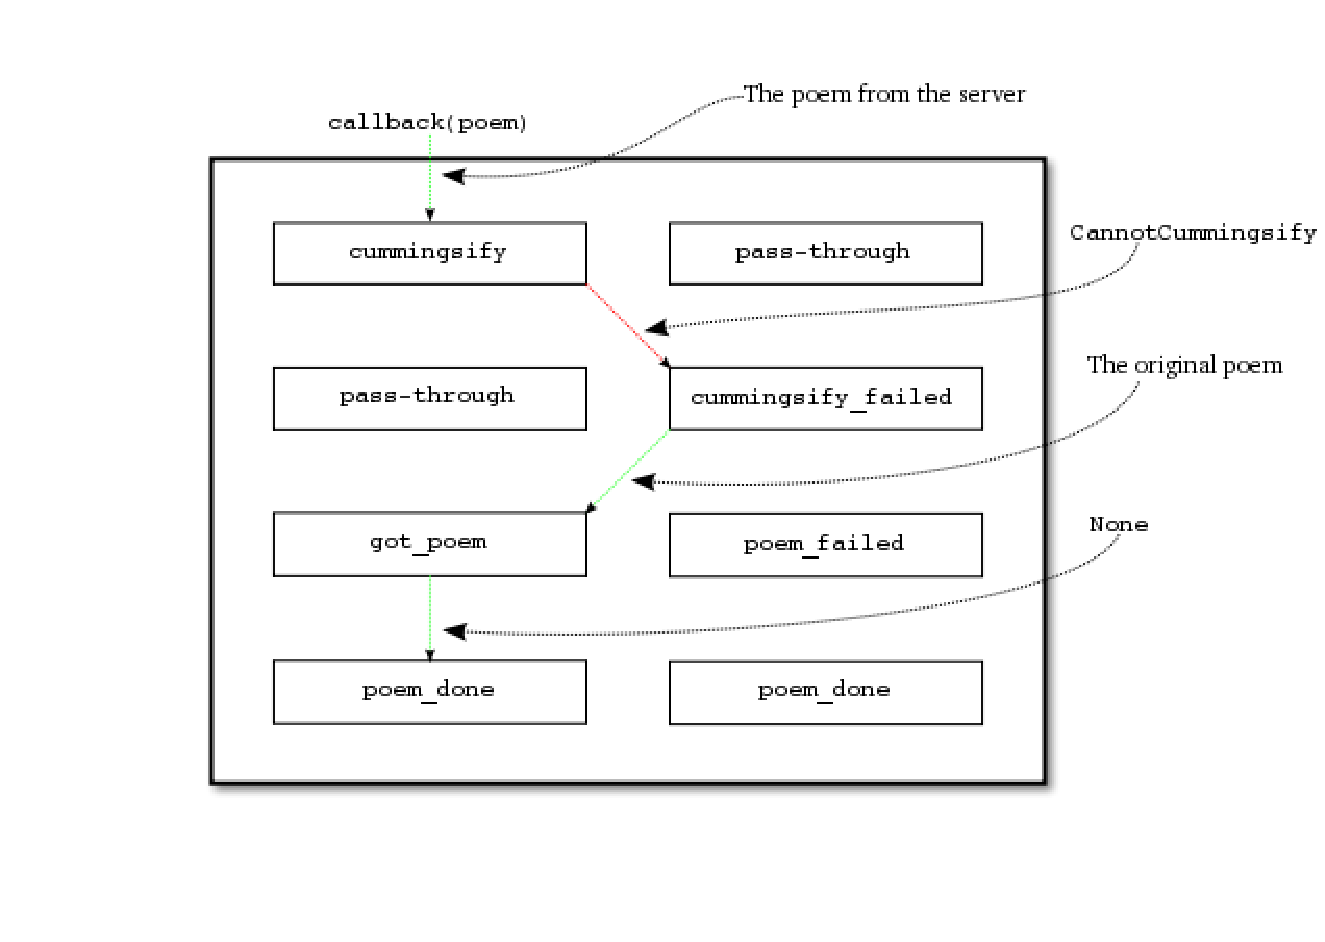
\includegraphics[width=0.8\textwidth]{images/deferred-10.pdf}
    \caption{Когда мы получаем ошибку CannotCummingsify\label{fig:deferred-10}}
\end{center}
\end{figure}

Таким образом, когда мы используем deferred'ы, 
иногда мы можем выбрать хотим ли мы использовать 
операторы try/except для управления исключениями или позволить deferred'м 
отправлять ошибки в errback.


\subsection{Резюме}


В главе 10 мы обновили наш поэтический клиент для 
того, чтобы использовать возможность Deferred 
маршрутизовать ошибки и результаты по цепи callback'в и errback'в. 
Хотя пример был достаточно искусственным, он проиллюстрировал 
как контролирующий поток в deferred'х переключается 
между callback и errback цепями взависимости от результата 
на каждой стадии.


Так что теперь мы знаем все, что можно знать про deferred'ы, верно? 
Нет еще! Мы будем исследовать остальные особенности deferred'в в 
следующей части. Но сначала, мы поедем немного в объезд и, в главе 11, 
реализуем Twisted версию нашего поэтического сервера.  

\subsection{Упражнения}

\begin{enumerate}

\item На рисунке \ref{fig:deferred-10} показан один из четырех 
возможных способах активизации deferred'а в клиенте 5.1. Нарисуйте 
три других. 

\item Используйте \href{http://github.com/jdavisp3/twisted-intro/blob/master/twisted-deferred/deferred-simulator.py#L1}{deferred simulator} для эмулирования всех возможных активизаций для клиетов 5.0 и 5.1. 
Для начала, эта программа может представлять случай, где функция try\_to\_cummingsify 
успешно завершается в клиенте 5.0: 

\begin{scriptsize}\begin{verbatim}
r poem p
r None r None
r None r None
\end{verbatim}\end{scriptsize}

\end{enumerate}
